\ifx\wholebook\relax \else

\documentclass[b5paper]{ctexart}
\usepackage[nomarginpar
  %, margin=.5in
]{geometry}

\addtolength{\oddsidemargin}{-0.05in}
\addtolength{\evensidemargin}{-0.05in}
\addtolength{\textwidth}{0.1in}

\usepackage[cn]{../prelude}

\setcounter{page}{1}

\begin{document}

\title{数字}

\author{刘新宇
\thanks{{\bfseries 刘新宇} \newline
  Email: liuxinyu95@gmail.com \newline}
  }

\maketitle
\fi

\markboth{数字}{编程中的数学}

\ifx\wholebook\relax
\chapter{数字}
\numberwithin{Exercise}{chapter}
\fi

\epigraph{数能引导我们走向真理}{——柏拉图写给老师苏格拉底的信}

\section{数的诞生}

\begin{wrapfigure}{R}{0.3\textwidth}
%\begin{figure}[htbp]
 \centering
 \includegraphics[scale=0.36]{img/clay-envelope.jpg}
 \caption{卢浮宫陈列的乌鲁尔时期的计数陶罐和一组计数陶球。}
 \label{fig:clay-token}
%\end{figure}
\end{wrapfigure}

\textbf{自}从人类进化开始,数的概念就伴随着我们。有人认为,数直接催生了人类的语言和文字。我们的祖先在长期的狩猎、采集活动中,逐渐掌握了数的概念。
最早可能是简单的数数,如数清果实的数量。随着文明的发展,人们逐渐开始进行物品交易。交易的数量逐渐增长,这就需要采用助记工具来处理更大的数。
考古发现在今天的伊朗一带,人们在公元前4000年左右开始使用陶制的小球来辅助计数。比如用两个刻有十字的小球代表两只羊,同时还有代表十只羊,二十只羊的不同小球。
为了防止忘记或者篡改数过的数目,人们还把这些小球放在陶罐中用泥土封存起来。图\ref{fig:clay-token}是乌鲁克时期的陶制计数罐和小球\cite{wiki-number}。
交易过程中,人们可以通过这些工具掌握货物的数量\cite{trip-to-number-kingdom}。

% 乌鲁克(Uruk)

\textbf{然}而随着交易的增加和数目的增大,这样的陶罐和小球就不够方便了。大约公元前3500年,美索不达米亚的苏美尔人开始在泥板上刻划符号来记录交易。将泥板烤硬后就可以方便保存。人们在这一时期用坚硬的笔在泥板上刻出不同的符号,同时表示交易的物品和数量。比如用一个象形符号表示五头牛,而用另一个象形符号表示十只羊。

\textbf{数}的更大进步发生在公元前3100年左右,从出土的泥板中,我们发现苏美尔人开始将数字从它所代表的物品中抽象出来。人们不再使用一个符号同时表示物品和数量,而是用一个符号表示数量,接下来用另一个符号表示物品。例如先用一个符号表示五,然后跟上一个牛的象形符号表示五头牛;而表示五只羊的时候,人们用同样的符号表示五,然后再跟上一个羊的符号。这些泥板上的符号逐渐演变成了古巴比伦的楔形文字。

%\begin{wrapfigure}{R}{0.5\textwidth}
\begin{figure}[htbp]
 \centering
 \subcaptionbox{巴比伦楔形文字中的数字\cite{wiki-babylonian-num}}[0.45\linewidth]{
   \includegraphics[scale=0.36]{img/Babylonian_numerals.jpg}} \quad \quad
 \subcaptionbox{抽象的数字三}[0.45\linewidth]{
   \includegraphics[scale=0.21]{img/abstract-num.png}}
 %\captionsetup{labelformat=empty}
 \caption{古文字中的数字}
 \label{fig:babylonian-num}
 \label{fig:abstract-num}
\end{figure}
%\end{wrapfigure}

\textbf{产}生抽象的数是智慧生命思维的结果。人们发现三个鸡蛋、三棵树、三个陶罐都可以用数字三来表示。这是一种强大的工具。从此,我们可以对抽象的数字进行操作,然后再把结果应用到各种具体事物上。例如我们可以把抽象的数字三加上一得到四,从而知道捡拾三个鸡蛋后再捡拾到一个鸡蛋会得到四个鸡蛋。同时我们也知道烧制三个陶罐后再烧制一个陶罐会得到四个陶罐。人们逐渐从解决单一问题发展到解决一类问题。


\textbf{生}产劳动中从数数开始,我们的老祖先逐渐发展出了操作抽象数字的方法,包括数字的加法、减法,更为强大的乘法,以及用于分配事物的除法。在丈量分割土地,计算谷物容量时,又逐渐将抽象的数和几何量联系起来。各个文明几乎分别独立地发现了数与形的内在规律。我们发现古埃及、古希腊、古中国都各自发现了毕达哥拉斯定理(勾股定理),古埃及人把它应用于建造金字塔这样的伟大工程。从现代文明追根溯源,我们可以说自然数是数学和自然科学这条长河的源头。德国数学家克罗内克说“上帝创造了自然数,其余都是人的工作。”\footnote{一说为整数。}

% 克罗内克(Kronecker)

\section{皮亚诺自然数公理}
\index{皮亚诺公理(Peano Axioms)}
\index{归纳公理(Axiom of induction)}

% 皮亚诺公理(Peano Axioms)
古希腊的欧几里得在他的伟大著作《几何原本》中开创了公理化方法。他用五条公理和五条公设作为基石,精心构建一条一条定理的证明。每一个结论都仅仅使用公理和此前已经证明的定理。最终构建出了叹为观止的几何大厦。然而对于自然数,长期以来人们却没有建立起它的公理化形式系统。也许人们一直认为自然数的结论是直观和显而易见的。直到1889年,意大利数学家皮亚诺才为自然数建立起严格的公理化系统。这就是著名的皮亚诺公理。也许是上帝的巧合,欧几里得几何公理有五条,皮亚诺公理也有五条:

\begin{enumerate}
\item 0是自然数。即:$0 \in N$;
\item 每个自然数$n$都有它的下一个自然数$n'$,称为它的后继。记为$n' = succ(n)$;
\end{enumerate}

似乎仅仅有这两条公理,我们已经能够定义出无穷无尽的自然数了,从0开始,下一个是1,下一个是2,……,接下来是某个$n$,下一个是$n+1$,……以至无穷。但是好挑刺的数学家给出了一个反例:考虑只有两个元素$\{0, 1\}$组成的数字系统,定义1的后继为0,0的后继为1。这样也满足上面的两条公理,却不是我们想像中的自然数

为此我们还需要第三条皮亚诺公理来排除这种情况。

\begin{enumerate}
  \setcounter{enumi}{2}
  \item 0不是任何自然数的后继。即$\forall n \in N: n' \neq 0$;
\end{enumerate}

仅仅有这三条公理就够了么?我们还可以给出一个反例:考虑有限元素$\{0, 1, 2\}$组成的数字系统,定义0的后继是1,1的后继是2,2的后继还是2。这样也能满足上述三条公理。为此我们还需要第四条皮亚诺公理。

\begin{enumerate}
  \setcounter{enumi}{3}
  \item 不同的自然数有不同的后继。或者说,如果两个自然数的后继相同,那么它们相等。即任意$n, m \in N$若$n' = m'$则$n = m$;
\end{enumerate}

但是,仅仅用这四条公理仍然不够,因为可以存在这样的反例:考虑集合\{0, 0.5, 1, 1.5, 2, 2.5, ...\},定义0的后继是1、1的后继是2……,0.5的后继是1.5、1.5的后继是2.5……但0.5不是任何元素的后继。为了排除这种“不可达”元素,还需要最后一条皮亚诺公理。

\begin{enumerate}
  \setcounter{enumi}{4}
  \item 如果自然数的某个子集包含0,并且其中每个元素都有后继元素。那么这个子集就是全体自然数。符号表示为:若$S \subseteq N$,$0 \in S$且$\forall n \in S$有$n' \in S$则$S = N$。
\end{enumerate}

% 归纳公理(Axiom of induction)
为什么公理5可以排除掉上述反例呢?考虑$\{0, 0.5, 1, 1.5, 2, 2.5, ...\}$的一个子集$\{0, 1, 2, ...\}$。它包含0,并且每个元素都有后继元素,但是它不等于原集合。因为1.5、2.5……都不在这个子集中。所以它不满足第五条公理。公理五还有另外一个响亮的名字——归纳公理,它可以这样等价地描述:

\begin{enumerate}
  \setcounter{enumi}{4}
  \item 任意关于自然数的命题,如果证明了它对自然数0是对的,又假定它对自然数$n$为真时,可以证明它对$n'$也真,那么命题对所有自然数都真。(这条公理保证了数学归纳法的正确性)
\end{enumerate}

以上就是完整的五条皮亚诺公理,用它们可以构建出一阶算术系统,也称为皮亚诺算术系统\footnote{也有人规定自然数从1开始,而不是0开始。在皮亚诺当年的著作中,五条公理的顺序与此不同,其中第五条归纳公理被写在第三的位置上。}。

%\begin{wrapfigure}{R}{0.35\textwidth}
\begin{figure}[htbp]
 \centering
 \includegraphics[scale=0.2]{img/Peano.jpg}
 %\captionsetup{labelformat=empty}
 \caption{朱塞佩$\cdot$皮亚诺(Giuseppe Peano)1858 - 1932。}
 \label{fig:Peano}
\end{figure}
%\end{wrapfigure}

朱塞佩·皮亚诺1858年8月27日生于意大利库内奥(Cuneo)附近的斯宾尼塔(Spinetta)村。这是位于意大利北部都灵附近的农村。他出生的时候,正值意大利统一。1876年皮亚诺考入都灵大学学习,1880年毕业后就留校任教。皮亚诺最开始讲授微积分课程,1887年他和克罗西奥(Carola Crosio)结婚。1886年起,皮亚诺还同时担任都灵军事学院的教授。从19世纪80年代起,皮亚诺开始研究数理逻辑,并致力于数学基础的构建工作。他撰写了《数学公式汇编》这本巨著,力图把所有的数学成果都用形式化的方法汇集起来。这本书可以说为数学的严密化奠定了基础。1900年在第二届国际数学家大会上,罗素遇到了皮亚诺,他在自传(1951)中说\cite{M-Kline-2007}:

“这次大会是我的精神生活的一个转折点,因为在那里我遇到了皮亚诺。在此之前,我已经听说过他的名字,也知道他的一些工作。我突然明白了,他的符号提供了我多年来一直试图寻找的分析的工具,而且从他那里我获得了一直以来想要从事的工作的一种新的有效的技术。”

皮亚诺强烈地影响了罗素和怀特海合著的《数学原理》一书,对早期的计算理论起了重要的作用。皮亚诺最初用法语发表研究著作,但他对自然语言固有的歧义感到不满。为了解决这个问题,他于1900年左右发明了一套没有歧义的统一语言,称为“无屈折拉丁语”。这门语言后来被称为“国际语”\footnote{国际语的英文为Interlingua,它和世界语(Esperanto)是两种不同的人造语言}。皮亚诺努力推广他的新语言,但是事实并不如他所愿,几乎没有人愿意读他用国际语重写的《数学公式汇编》。相反倒是他早期的法语著作使数学家的观点发生了深刻的变化,尤其对法国的布尔巴基学派的纲领,产生了很大影响。后者包含了一大批20世纪世界顶级的数学家,如安德烈·韦伊、亨利·嘉当等。1932年4月20日,皮亚诺因心脏病逝世于都灵。

\section{自然数和计算机程序}
现代计算机系统和在其上构建的程序已经非常复杂宏伟了。人们并非是先建立了计算机程序的公理系统,然后演绎出这些成果的。而是先取得了应用的巨大成功,然后才逐渐将计算机科学的基石数学化、形式化、严谨化的。这种有趣的现象在人类历史上已经不是第一次了。牛顿和莱布尼茨在17世纪发展了微积分,然后在几代数学家的手里应用到了各种领域,包括流体力学,天文学等等。但是直到19世纪才由魏尔斯特拉斯、柯西等人将微积分的理论严格化\cite{M-Kline-2007}。

我们也模仿一下这样的过程,看看如何根据皮亚诺公理,用计算机程序定义自然数。在一个没有0、1、2、……这些数字的程序系统中,我们可以这样定义自然数\footnote{本书使用一种理想的计算机语言,并在每一章节的最后给出真实计算机语言的参考代码。}:

\begin{Haskell}
data Nat = zero | succ Nat
\end{Haskell}

%% \[
%% N \triangleq zero | succ(N)
%% \]

这一定义说:一个自然数或者为零,或者是另一自然数的后继。符号“|”表示互斥的关系。它自然蕴含了零不是任何自然数后继这一公理。在此基础上,我们可以进一步定义出自然数的加法。

\index{自然数的加法}

\begin{Haskell}
a + zero = a
a + (succ b) = succ (a + b)
\end{Haskell}

加法定义包含两部分。首先任何自然数和零相加等于它本身;并且某个自然数和另一个数的后继相加,等于这两个数相加的后继。写成数学符号为:

\be
\begin{array}{l}
a + 0 = a \\
a + b' = (a + b)'
\end{array}
\ee

我们来验证一下2+3。自然数2为succ(succ zero),而3为succ(succ(succ zero))。根据加法的定义2+3为:

\begin{Haskell}
  succ(succ zero) + succ(succ(succ zero))
= succ(succ(succ zero) + succ(succ zero))
= succ(succ(succ(succ zero) + succ zero))
= succ(succ(succ(succ(succ zero) + zero)))
= succ(succ(succ(succ(succ zero))))
\end{Haskell}

最终结果的确是零的五重后继,也就是5。从零开始一次一次地套用后继函数很麻烦。如果要表示100,这种记法要写很多行并且容易出错。为此,我们用下面的简单记法表示自然数$n$:

\be
n = foldn(zero, succ, n)
\ee

\index{自然数的叠加}
它表示从零开始,不断叠加使用succ函数$n$次。$foldn$函数可以具体实现如下:

\be
\begin{array}{l}
foldn(z, f, 0) = z \\
foldn(z, f, n') = f(foldn(z, f, n))
\end{array}
\label{eq:foldn}
\ee

$foldn$定义了在自然数上的一种操作,只要令$z$为$zero$,令$f$为$succ$就可以实现叠加后继若干次,从而获得某个特定的自然数。我们可以用前几个自然数验证一下:

\begin{Haskell}
foldn(zero, succ, 0) = zero
foldn(zero, succ, 1) = succ(foldn(zero, succ, 0)) = succ zero
foldn(zero, succ, 2) = succ(foldn(zero, succ, 1)) = succ(succ zero)
...
\end{Haskell}

\index{自然数的乘法}
定义好加法之后,我们再来定义自然数的乘法:

\begin{Haskell}
a *'.'* zero = zero
a *'.'* (succ b) = a *'.'* b + a
\end{Haskell}

这里使用了刚定义好的加法。这一定义写成数学符号为:

\be
\begin{array}{l}
a \cdot 0 = 0 \\
a \cdot b' = a \cdot b + a
\end{array}
\ee

\begin{figure}[htbp]
%\begin{wrapfigure}{R}{0.4\textwidth}
\centering
\begin{tikzpicture}[scale=0.8]
\filldraw[fill=gray, draw=black, pattern=north west lines] (0, 0) rectangle (2, 1)
    (2, 0) rectangle (3, 1);
\draw (3, 0) rectangle (4.5, 1);
\draw (0, -1) rectangle (2, -2);
\filldraw[fill=gray, draw=black, pattern=north west lines] (2, -1) rectangle (3, -2)
    (3, -1) rectangle (4.5, -2);
\end{tikzpicture}
\caption{加法结合律:上下面积相等}
%\end{wrapfigure}
\end{figure}

\index{加法结合律}
与通常的观念不同,加法和乘法的交换律、结合律既不是公理,也不是公设。它们都是定理,可以用皮亚诺公理和定义证明。以加法结合律为例。结合律是说$(a + b) + c= a + (b + c)$。我们先证明当$c=0$时它是对的。根据加法定义的第一条规则:

\[
\begin{array}{rl}
(a + b) + 0 & = a + b \\
            & = a + (b + 0)
\end{array}
\]

然后是递推步骤,假设$(a + b) + c = a + (b + c)$成立,我们要推出$(a + b) + c' = a + (b + c')$。

\[
\begin{array}{rlr}
(a + b) + c' & = (a + b + c)' & \text{加法定义的规则二,反向} \\
             & = (a + (b + c))' & \text{递推假设} \\
             & = a + (b + c)' & \text{加法定义的规则二} \\
             & = a + (b + c') & \text{加法定义的规则二,反向}
\end{array}
\]

这样就证明了加法的结合律。但加法交换律的证明却并不简单,本书附录给出了完整的证明。

%\begin{wrapfigure}{R}{0.4\textwidth}
\begin{figure}[htbp]
\centering
\begin{tikzpicture}[scale=0.8]
\draw (0, 0) rectangle (2, 1)
    (2, 0) rectangle (3, 1);
\draw (0, -1) rectangle (1, -2)
    (1, -1) rectangle (3, -2);
\end{tikzpicture}
\caption{加法交换律:将上方的图形倒过来看,或者在镜中看。}
\end{figure}
%\end{wrapfigure}

\begin{Exercise}\label{ex:Peano-axiom}
\Question{定义0的后继为1,证明对于任何自然数都有$a \cdot 1 = a$}
\Question{证明乘法分配律。}
\Question{证明乘法结合律和交换律。}
\Question{如何利用皮亚诺公理验证3 + 147 = 150?}
\Question{试给出乘法分配律,乘法结合律,和乘法交换律的几何解释。}
\end{Exercise}

\begin{Answer}[ref={ex:Peano-axiom}]
\Question{定义0的后继为1,证明对于任何自然数都有$a \cdot 1 = a$

首先用数学归纳法证明$0 + a = a$这个结论,见附录\textbf{加法交换律的证明}。然后:
\[
\begin{array}{rlr}
a' \cdot 1 & = a' \cdot 0' & \text{定义0的后继为1} \\
           & = a' \cdot 0 + a' & \text{乘法定义规则二} \\
           & = 0 + a' & \text{乘法定义规则一} \\
           & = a' & \text{此前证明的结论}
\end{array}
\]
}
\Question{证明乘法分配律。

\begin{proof}
可以用数学归纳法证明左侧的分配律$c(a + b) = ca + cb$。首先是$b = 0$的情况:

\bre
c(a + 0) & = & ca & \text{加法规则一} \\
         & = & ca + 0 & \text{反向用加法规则一} \\
         & = & ca + c0 & \text{反向用乘法规则一} \\
\ere

递推假设$c(a + b) = ca + cb$,接下来证明$c(a + b') = ca + cb'$

\bre
c(a + b') & = & c(a + b)' & \text{加法规则二} \\
          & = & c(a + b) + c & \text{乘法规则二} \\
          & = & ca + cb + c & \text{递推假设} \\
          & = & ca + (cb + c) & \text{加法结合律} \\
          & = & ca + cb' & \text{反向用乘法规则二} \\
\ere
\end{proof}
}
\Question{证明乘法结合律和交换律。

我们只证明乘法结合律$(ab)c = a(bc)$,乘法交换律的证明则给出一个提纲。利用数学归纳法,首先是$c = 0$的情况:

\bre
(ab)0 & = & 0 & \text{乘法规则一} \\
      & = & a0 & \text{反向用乘法规则一} \\
      & = & a(b0) & \text{反向用乘法规则一} \\
\ere

递推假设$(ab)c = a(bc)$,接下来要证明$(ab)c' = a(bc')$

\bre
(ab)c' & = & (ab)c + ab & \text{乘法规则二} \\
       & = & a(bc) + ab & \text{递推假设} \\
       & = & a(bc + b) & \text{上题证明的分配律} \\
       & = & a(bc') & \text{反向用乘法规则二} \\
\ere

证明乘法交换律可以分为三步,都使用数学归纳法。首先证明$1a = a$,然后再证明右侧的分配律$(a + b)c = ac + bc$,最后再证明交换律。
}
\Question{如何利用皮亚诺公理验证3 + 147 = 150?

我们先看看经典的2 + 2 = 4是怎么证明的:

\bre
2 + 2 & = & 0'' + 0'' & \text{2是0的两次后继} \\
      & = & (0'' + 0')' & \text{加法定义规则二} \\
      & = & ((0'' + 0)')' & \text{加法定义规则二} \\
      & = & ((0'')')' & \text{加法定义规则一} \\
      & = & 0'''' = 4 & \text{0的4次后继} \\
\ere

显然用这个方法证明3 + 147 = 150的话太冗长了,我们可以用先前证明的加法交换律证明147 + 3 = 150会容易一些。另一个方法是通过数学归纳法证明$3 + a = a'''$。
}
\Question{试给出乘法分配律,乘法结合律,和乘法交换律的几何解释。

%\begin{figure}[htbp]
\begin{center}
 \includegraphics[scale=0.4]{../appendix/answer/img/geometric-arithmetic}
 \captionof{figure}{乘法交换律、结合律、分配律的几何解释}
 \label{fig:geometric-arithmetic}
\end{center}
%\end{figure}
}
\end{Answer}

\section{自然数的结构}
有了加法和乘法,我们就可以定义更复杂的计算。第一个例子是累加:$0 + 1 + 2 + ... $

\be
\begin{array}{l}
sum(0) = 0 \\
sum(n + 1) = (n + 1) + sum(n)
\end{array}
\ee

第二个例子是阶乘$n!$

\be
\begin{array}{l}
\textit{fact}(0) = 1 \\
\textit{fact}(n + 1) = (n + 1) \cdot \textit{fact}(n)
\end{array}
\ee

这两个例子非常相似。尽管人工智能日新月异地发展,智慧生命和智能机器的一大区别就是能否“跳出系统”,到更高的层次进行抽象。这是我们人类心智中最强大、神秘、复杂、难以捉摸的一部分\cite{GEB}。

我们发现累加和阶乘都有一个针对自然数零的起始值,累加始自零,阶乘始自一。针对递归情况,它们都将某一操作应用到一个自然数和它的后继上。累加是$n' + sum(n)$,阶乘是$n' \cdot \textit{fact}(n)$。如果我们把起始值抽象为$c$,把递归中的操作抽象为$h$,就可以用一个统一的形式概括累加和阶乘。

\be
\begin{array}{l}
f(0) = c \\
f(n + 1) = h(f(n))
\end{array}
\ee

这是一个在自然数上的递归结构。我们观察一下它在前几个自然数上的表现。

\vspace{5mm}
\begin{tabular}{l|l}
$n$ & $f(n)$ \\
\hline
0 & $c$ \\
1 & $f(1) = h(f(0)) = h(c)$ \\
2 & $f(2) = h(f(1)) = h(h(c))$ \\
3 & $f(3) = h(f(2)) = h(h(h(c)))$ \\
... & ... \\
$n$ & $f(n) = h^n(c)$
\end{tabular}
\vspace{5mm}

其中,$h^n(c)$表示我们叠加在$c$上重复进行$n$次$h$操作。它是\textbf{原始递归}形式的一种(\cite{Bird97},第5页)。更进一步,如果观察此前我们在(\ref{eq:foldn})定义的函数$foldn$,就会发现它们之间的关系:

\be
f = foldn(c, h)
\ee

细心的读者会观察到,我们最初定义的$foldn$带有三个参数,为什么这里只有两个了呢?实际上我们可以写成$f(n) = foldn(c, h, n)$。当我们仅传递给三元函数$foldn$前两个参数,它实际上就成为了接受一个自然数为参数的一元函数了。我们可以这样看待它:$foldn(c, h)(n)$。

我们称$foldn$为自然数上的叠加($fold$)操作。令$c$为$zero$,$h$为$succ$,我们就得到了自然数。如同上面的表格,我们可以得到一个序列:

\[
zero, succ(zero), succ(succ(zero)), ... succ^n(zero), ...
\]

如果$c$不是$zero$,$h$不是$succ$,则$foldn(c, h)$就描述了和自然数同构\footnote{同构(isomorphism)的严格定义将在第3章给出,这里泛指结构上的一种对应。}的某种事物。我们来看几个例子:

\[
(+ m) = foldn(m, succ)
\]

这个例子描述了将自然数$n$增加$m$的操作,将它依次作用到自然数上可以产生和自然数同构的序列$m, m + 1, m + 2, ..., n + m, ...$

\[
(\cdot m) = foldn(0, (+ m))
\]

这个例子描述了将自然数$n$乘以$m$的操作,将它依次作用到自然数上可以产生和自然数同构的序列$0, m, 2m, 3m, ..., nm, ...$

\[
m^{()} = foldn(1, (\cdot m))
\]

这个例子描述了对自然数$m$取$n$次幂的操作,将它依次作用到自然数上可以产生和自然数同构的序列$1, m, m^2, m^3, ..., m^n, ...$

那么,我们思考出的这个抽象工具$foldn$能否描述累加和阶乘呢?我们观察下面的这个表格:

\vspace{5mm}
\begin{tabular}{r|l|l|l|l|l|l}
$n$ & 0 & 1 & 2 & 3 & ... & $n'$ \\
\hline
$sum(n)$ & 0 & 1 + 0 = 1 & 2 + 1 = 3 & 3 + 3 = 6 & ... & $n' + sum(n)$ \\
\hline
$n!$ & 1 & 1 $\times$ 1 = 1 & 2 $\times$ 1 = 2 & 3 $\times$ 2 = 6 & ... & $n' \cdot (n!)$
\end{tabular}
\vspace{5mm}

这里的关键问题是$h$必须是个二元操作,它能够对$n'$和$f(n)$进行运算。为此,我们将$c$也定义为一个二元数$(a, b)$\footnote{在计算机程序中,也称为二元组(tuple),或者对(pair)。}。然后针对二元数$(a, b)$定义某种类似“succ”的操作。最终为了获取结果,我们还需要要定义从二元数中抽取$a$和$b$的函数:

\be
\begin{array}{l}
1st (a, b) = a \\
2nd (a, b) = b
\end{array}
\ee

这样我们就可以定义累加和阶乘了。首先是累加的定义:

\[
\begin{array}{lr}
c = (0, 0) & \text{二元数的起始值} \\
h (m, n) = (m', m' + n) & \text{第一个数取后继,第二个数加第一个数的后继} \\
sum = 2nd \circ foldn(c, h) \\
\end{array}
\]

我们看看,从起始值$(0, 0)$开始,会怎样一步一步递推出累加的结果。

\vspace{5mm}
\begin{tabular}{r|l|l}
$(a, b)$ & $(a', b') = h (a, b)$ & $b'$\\
\hline
(0, 0) & (0 + 1 = 1, 1 + 0 = 1) = (1, 1) & 1 \\
(1, 1) & (1 + 1 = 2, 2 + 1 = 3) = (2, 3) & 3 \\
(2, 3) & (2 + 1 = 3, 3 + 3 = 6) = (3, 6) & 6 \\
... & ... & ... \\
$(m, sum(m))$ & $(m + 1, m + 1 + sum(m))$ & $sum(m + 1)$
\end{tabular}
\vspace{5mm}

类似地,我们用$foldn$定义出阶乘。

\[
\begin{array}{lr}
c = (0, 1) & \text{阶乘的起始值} \\
h (m, n) = (m', m'n) & \text{阶乘的递推} \\
fact = 2nd \circ foldn(c, h) \\
\end{array}
\]

\index{函数组合}
在累加和阶乘的定义中,我们使用了符号“$\circ$”点来连接两个函数$2nd$和$foldn(c, h)$。我们称之为函数组合,$f \circ g$表示先将函数$g$应用到变量上,然后再将函数$f$应用到结果上。即$(f \circ g)(x) = f(g(x))$。

\index{斐波那契}
\begin{figure}[htbp]
 \centering
 \includegraphics[scale=0.35]{img/Fibonacci}
 %\captionsetup{labelformat=empty}
 \caption{比萨的列奥纳多(斐波那契)1175-1250}
 \label{fig:Fibonacci}
\end{figure}

为了展示这一抽象工具的强大,我们再来看一个例子:斐波那契数列。这一数列是用中世纪数学家比萨的列奥纳多命名的。斐波那契来自拉丁文filius Bonacci意思是波那契之子。斐波那契的父亲当时是商人,在北非以及地中海一带经商,斐波那契逐渐向当地阿拉伯人学习了印度——阿拉伯的数字系统并通过他的著作《算盘书》(Liber Abaci)将其介绍到欧洲。中世纪的欧洲一直使用罗马数字系统,我们今天在一些钟表盘上仍然可以看到罗马数字。例如2018年的罗马数字表示为MMXVIII,其中一个M代表1000,两个M代表2000,X代表10,V表示5,三个I表示3。把这些加起来得到2018。斐波那契引入欧洲的是我们今天仍然使用的位值制十进制系统。它使用了印度数学发明的零,不同的数字在不同的位置上含义不同。这一先进的数字系统极大地方便了计算,广泛应用在记账、利息、汇率等方面。《算盘书》更是对欧洲的数学复兴产生了深远的影响。

斐波那契数列来自《算盘书》中的一个问题:兔子在出生两个月后,就有繁殖能力,一对兔子每个月能生出一对小兔子来。如果所有兔子都不死,那么一年以后可以繁殖多少对兔子?开始时有一对兔子。第一个月小兔尚未具备繁殖能力,所以仍然只有一对兔子。第二个月它们生下一对小兔,共有两对。第三个月大兔子又生下一对小兔,而上月生的小兔还在成长,总共有2+1=3对。第四个月有两对大兔子产下两对小兔,加上原有的三对兔子,总共有3+2=5对。按照这样,我们可以得到一个序列

1, 1, 2, 3, 5, 8, 13, 21, 34, 55, 89, 144, ...

\begin{figure}[htbp]
 \centering
 \subcaptionbox{正方形的边长组成了斐波那契序列}[0.45\linewidth]{
     \includegraphics[scale=0.4]{img/fibonacci_spiral}}
 \subcaptionbox{深色:成兔,浅色:小兔}[0.45\linewidth]{
     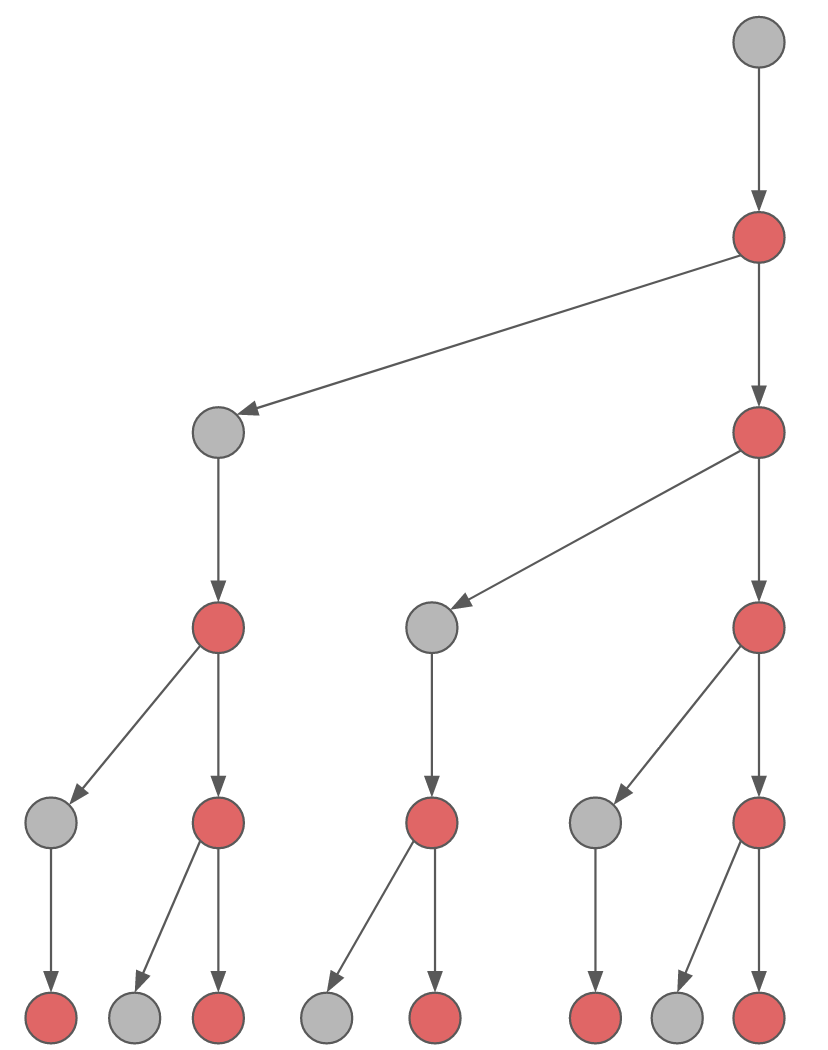
\includegraphics[scale=0.3]{img/Fibonacci-rabbits}}
 %\captionsetup{labelformat=empty}
 \caption{斐波那契序列展开}
 \label{fig:fibonacci_spiral}
 \label{fig:Fibonacci-rabbits}
\end{figure}

\index{斐波那契数列}
这个数列很有规律,从第三项后,任何一项都等于前两项的和。我们可以这样思考它的原理,如果前一个月有$m$对兔子,这个月有$n$对兔子,那么增加的一定都是新产下的小兔,共有$n-m$对,而剩下的都是成年兔子,共$m$对。到下个月时,这$n-m$对小兔刚刚成熟,而$m$对成兔又产下了$m$对小兔。所以下个月的兔子总数等于小兔加上成兔为:$(n - m) + m + m = n + m$对。根据这一推理,我们可以给出斐波那契数列的递归定义:

\be
\begin{array}{l}
F_0 = 0 \\
F_1 = 1 \\
F_{n+2} = F_n + F_{n+1}
\end{array}
\ee

通常将斐波那契数列的起始值定义为0和1\footnote{如果起始值是1和3,我们就得到了卢卡斯数列1, 3, 4, 7, 11, 18, ...}。注意到斐波那契数列的起始值是一对自然数,并且递推关系也是一对值。我们可以利用抽象工具$foldn$给出下面的定义\footnote{在介绍康托尔的无穷概念时,我们会给出另一个斐波那契数列的定义。}:

\be
\begin{array}{l}
F = 1st \circ foldn((0, 1), h) \\
h (m, n) = (n, m + n)
\end{array}
\ee

也许读者会好奇,真实的计算机程序能实现这样的定义么?这是不是太理想化了?下面是一段的Haskell语言的程序代码\footnote{2010年后,Haskell中不再允许使用n+k形式的模式匹配。},执行\texttt{fib 10}会输出斐波那契数55\footnote{一行代码输出前100个斐波那契数的例子:\newline\texttt{take 100 \$ map fst \$ iterate ($\lambda$(m, n)->(n, m + n)) (0, 1)}}。

\begin{Haskell}[frame = single]
foldn z _ 0 = z
foldn z f n = f (foldn z f (n - 1))

fib = fst . foldn (0, 1) h where
  h (m, n) = (n, m + n)
\end{Haskell}

\begin{Exercise}\label{ex:foldn}
\Question{使用$foldn$定义平方$()^2$。}
\Question{使用$foldn$定义$()^m$,计算给定自然数的$m$次幂。}
\Question{使用$foldn$定义奇数的和。它会产生怎样的序列?}
\Question{地面上有一排洞(无限多个),一只狐狸藏在某个洞中。每天狐狸会移动到相邻的下一个洞里。如果每天只能检查一个洞,请给出一个捉到狐狸的策略,并证明这个策略有效。如果狐狸每天移动的不止一个洞呢\cite{Gusen2014}?}
\end{Exercise}

\begin{Answer}[ref={ex:foldn}]
\Question{使用$foldn$定义平方$()^2$。

可以利用递推关系$(n+1)^2 = n^2 + 2n + 1$来定义平方:

\[
()^2 = 2nd \circ foldn\ (0, 0)\ h
\]

其中$h$接受一对值$(i, s)$,分别代表自然数$i$和它的平方$s$。它将第一个值递增1,然后利用平方展开式求出下一个平方数。

\[
h\ (i, s) = (i + 1, s + 2i + 1)
\]
}
\Question{使用$foldn$定义$()^m$,计算给定自然数的$m$次幂。

一种简单的方法是借助第一章中定义的$m^{()} = foldn(1, (\cdot m))$来定义$()^m$:

\[
()^m = 2nd \circ foldn\ (0, 0)\ h
\]

其中

\[
h\ (i, b) = (i + 1, (i + 1)^m)
\]

这看起来有些奇怪,所有中间计算都被直接丢掉了。另一种方法是利用牛顿二项式定理:

\[
(n + 1)^m = n^m + \binom{m}{1} n^{m-1} + ... + \binom{m}{m-1} n + 1
\]

这样就建立了递推关系:

\[
(n)^m = 2nd(foldn\ (1, 1)\ h\ (n - 1))
\]

其中

\[
h (i, x) = (i + 1, C \cdot X)
\]

这里$C \cdot X$是二项式系数和各次幂的点积$C \cdot X = \sum c_j x_j$。各次幂可以通过对$x$不断除以$i$求出,二项式定理的系数可以由帕斯卡三角形逐行递推得到。下面是综合在一起的例子程序:

\lstset{frame=single}
\begin{Haskell}
exp m n = snd $ foldn (1, 1) h (n - 1) where
  cs = foldn [1] pascal m
  h (i, x) = (i + 1, sum $ zipWith (*) cs xs) where
    xs = take (m + 1) $ iterate (`div` i) x

pascal = gen [1] where
  gen cs (x:y:xs) = gen ((x + y) : cs) (y:xs)
  gen cs _ = 1 : cs
\end{Haskell}
}
\Question{使用$foldn$定义奇数的和。它会产生怎样的序列?

用$foldn$定义1 + 3 + 5 + ...为$2nd \circ foldn\ (1, 0)\ h$,其中:

\[
h\ (i, s) = (i + 2, s + i)
\]

如第一章中习题下的插图所示,奇数和总是平方数。
}
\Question{地面上有一排洞(无限多个),一只狐狸藏在某个洞中。每天狐狸会移动到相邻的下一个洞里。如果每天只能检查一个洞,请给出一个捉到狐狸的策略,并证明这个策略有效。如果狐狸每天移动的不止一个洞呢\cite{Gusen2014}?

不管狐狸在哪个洞中,我们只检查奇数洞1, 3, 5, ...必然会捉到狐狸。观察下面的表格

\btab{c|c|c|c|c}
1 & 3 & 5 & ... & 2m - 1 \\
\hline
m & m + 1 & m + 2 & ... & 2m - 1 \\
\etab

狐狸第一天在第$m$个洞中,解方程$m + k = 2k + 1$,得出当$k = m -1$天之后,我们恰好检查第$2m-1$洞,而狐狸恰好也在这个洞中。下面使用$foldn$展示了这一过程:

\[
\begin{array}{l}
fox\ m = foldn\ (1, m)\ h\ (m - 1) \\
\text{其中}: h\ (c, f) = (c + 2, f + 1) \\
\end{array}
\]

如果狐狸第一天在第$p$个洞中,每天移动$q$个洞,我们可以把这样的组合列为$(p, q)$的数偶。然后参考第6章无穷中的方法将其映射到自然数上进行枚举。
}
\end{Answer}

%\begin{wrapfigure}{R}{0.3\textwidth}
\begin{figure}[htbp]
 \centering
 \includegraphics[scale=0.2]{img/PWW.jpg}
 \caption{《无需语言的证明》封面局部}
 \label{fig:PWW}
\end{figure}
%\end{wrapfigure}

\section{自然数的同构}

\index{链表}
自然数不仅可以和自己的子集同构,例如奇偶数、平方数、斐波那契数,还可以和其它事物同构,包括计算机程序中的数据结构。下面是列表的定义:

\begin{Haskell}
data List A = nil | cons(A, List A)
\end{Haskell}

用数据结构的观点来解释,一个类型为A的列表或者为空,记为nil;或者包含两部分:一个含有类型A数据的节点,和一个包含剩余部分的子列表。函数cons把一个类型为A的元素和另一个类型为A的列表“链接”起来\footnote{名称cons来自Lisp的命名传统。}。图\ref{fig:linked-list}描述了一个含有6个节点的列表。

\begin{figure}[htbp]
\centering
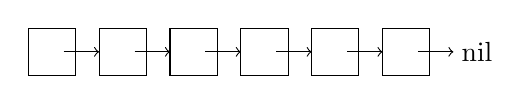
\begin{tikzpicture}[scale=3]
  \foreach \x in {-2, -1.7, ..., -0.4} {
    \draw (\x cm, 1cm) +(-0.1, -0.1) rectangle ++(0.1, 0.1);
    \draw[->] (\x cm, 1cm) +(0.05, 0) -- +(0.2, 0);
  }
  \draw (-0.2cm, 1cm) node {nil};
\end{tikzpicture}
\caption{Linked-list}
\label{fig:linked-list}
\end{figure}

由于这种特点,列表也被称为“链表”。传统的计算机程序中,链表通常定义为一个结构\footnote{很多情况下,列表中保存的数据类型是相同的。但也有异构类型的列表,例如Lisp中的列表。},例如:
\begin{lstlisting}
Node of A:
    key: A
    next: Node of A
\end{lstlisting}

我们也可以用自然数的同构来解释列表。根据皮亚诺公理一,nil相当于零;根据皮亚诺公理二,对于任何列表,我们都可以用cons,在其左侧链接一个类型为A的新元素。因此cons相当于自然数中的succ。这里的变化有两点。其一是列表携带类型A的元素,因而\texttt{cons(1, cons(2, cons(3, nil)))}和\texttt{cons(2, cons(1, cons(3, nil)))}和\texttt{cons(1, cons(4, cons(9, nil)))}以及\texttt{cons('a', cons('b', cons('c', nil)))}都是不同的列表。其二是与直觉不同,新元素不是加入到列表的右侧末尾,而是加入到左侧的头部。增长的方向是向左,而非向右。

用嵌套的cons表示较长的列表很不方便,我们将\texttt{cons(1, cons(2, cons(3, nil)))}简记为[1, 2, 3],用符号“:”表示cons。因此这一列表也可以写为1:[2, 3]或者1:(2:(3:nil))。针对A为字母的特殊情况,我们用带双引号的字符串来表示,例如用“hello”来简记表示['h', 'e', 'l', 'l', 'o']。

同构于自然数的加法,定义列表的连接运算如下:

\be
\begin{array}{l}
nil \doubleplus y = y \\
cons(a, x) \doubleplus y = cons(a, x \doubleplus y)
\end{array}
\ee

列表的连接运算包含两条规则。首先空列表和任何列表连接的结果仍然等于该列表本身;并且某个列表的“后继”和另一个列表相连接,等于这两个列表连接结果的后继。和自然数的加法对比,它们呈现出有趣的镜像对称形式。

\begin{figure}[htbp]
\begin{tabular}{r|l}
$nil \doubleplus y = y$ & $a + 0 = a$ \\
$cons(a, x) \doubleplus y = cons(a, x \doubleplus y)$ & $a + succ(b) = succ(a + b)$
\end{tabular}
%\caption{列表的连接和自然数的加法呈现镜像对称}
\end{figure}

\index{列表连接的结合律}
这种同构提示我们,可以利用递推公理证明列表连接的结合律。为了证明$(x \doubleplus y) \doubleplus z = x \doubleplus (y \doubleplus z)$,我们首先证明$x=nil$时的起始情况

\[
\begin{array}{lll}
(nil \doubleplus y) \doubleplus z & = y \doubleplus z & \text{列表连接定义的规则一} \\
 & = nil \doubleplus (y \doubleplus z) & \text{列表连接定义的规则一,反向}
\end{array}
\]

然后再证明递推情况。假设$(x \doubleplus y) \doubleplus z = x \doubleplus (y \doubleplus z)$,我们要证明$((a:x) \doubleplus y) \doubleplus z = (a:x) \doubleplus (y \doubleplus z)$。

\[
\begin{array}{rll}
((a:x) \doubleplus y) \doubleplus z & = (a:(x \doubleplus y)) \doubleplus z & \text{列表连接定义的规则二} \\
 & = a:((x \doubleplus y) \doubleplus z) & \text{列表连接定义的规则二} \\
 & = a:(x \doubleplus (y \doubleplus z)) & \text{递推假设} \\
 & = (a:x) \doubleplus (y \doubleplus z) & \text{列表连接定义的规则二,反向}
\end{array}
\]

这样我们就证明了列表连接操作的结合律。但是和自然数不同,列表不满足交换律\footnote{这也是我们避免使用加号“+”来表示列表连接的原因。但是很多编程语言使用了加号,这造成了一些潜在的问题。}。例如$[2, 3 ,5] \doubleplus [7, 11] = [2, 3, 5, 7, 11]$,但交换后的结果却是$[7, 11] \doubleplus [2, 3, 5] = [7, 11, 2, 3, 5]$。

考虑和自然数同构,我们也可以定义列表的抽象叠加操作。为此,我们仿照自然数定义一个抽象的起始值$c$,和一个抽象的二元运算$h$。这样就可以定义列表的递归形式:

\be
\begin{array}{l}
f(nil) = c \\
f(cons(a,x)) = h(a, f(x))
\end{array}
\ee

\index{列表的叠加}
进一步,令$f = foldr(c, h)$,就可以抽象出列表的叠加操作。我们将其命名为$foldr$以表明这种叠加操作是自右向左进行的。

\be
\begin{array}{l}
foldr(c, h, nil) = c \\
foldr(c, h, cons(a,x)) = h(a, foldr(c, h, x))
\end{array}
\ee

使用$foldr$,我们可以定义各种列表上的操作。例如我们可以把一个列表中的各个元素累加或累乘起来:

\be
\begin{array}{l}
sum = foldr(0, +) \\
product = foldr(1, \times)
\end{array}
\ee

以$sum$为例,首先是空列表:$sum(nil) = foldr(0, +, nil) = 0$;然后是若干个元素的列表:

\[
\begin{array}{rl}
sum([1, 3, 5, 7]) & = foldr(0, +, 1:[3, 5, 7]) \\
 & = 1 + foldr(0, +, 3:[5, 7]) \\
 & = 1 + (3 + foldr(0, +, 5:[7])) \\
 & = 1 + (3 + (5 + foldr(0, +, cons(7, nil)))) \\
 & = 1 + (3 + (5 + (7 + foldr(0, +, nil)))) \\
 & = 1 + (3 + (5 + (7 + 0))) \\
 & = 16
\end{array}
\]

我们还可以计算列表的长度。这本质上是把一个列表映射成自然数。

\be
\begin{array}{l}
h(a, n) = n + 1 \\
length = foldr(0, h)
\end{array}
\ee

这样我们就可以用$|x| = length(x)$来计算列表的长度。我们还可以用$foldr$定义连接操作$\doubleplus$:

\be
(\doubleplus y) = foldr(y, cons)
\ee

这相当于自然数的$(+m)$运算。类似自然数乘法,我们可以定义列表“乘法”,将一个“列表的列表”全部连接起来。

\be
concat = foldr(nil, \doubleplus)
\ee

例如:$concat([[1, 1], [2, 3, 5], [8]])$的结果是$[1, 1, 2, 3, 5, 8]$。我们接下来再用$foldr$定义两个重要操作:选择和逐一映射\footnote{和一一映射不同,这里的映射是单向的,例如从一个词语到它的字符长度的映射,其逆映射并不存在。}。选择也称为过滤,是根据某个条件选择列表中的元素组成一个新的列表。为此,我们需要引入条件表达式的概念\footnote{也称麦卡锡条件形式,是计算机科学家Lisp发明人约翰$\cdot$麦卡锡于1960年引入的。}。它通常写为$(p \mapsto f, g)$,也就是给定变量$x$,若条件$p(x)$成立,则结果为$f(x)$,否则为$g(x)$,我们也会用if $p(x)$ then $f(x)$ else $g(x)$来描述条件表达式。

\be
filter(p) = foldr(nil, (p \circ 1st \mapsto cons, 2nd))
\ee

为了理解这一定义,我们来看一个例子:从一组自然数中,选择出偶数

\[filter(even, [1, 4, 9, 16, 25])\]

和$sum$的例子类似,首先是一系列的展开过程,$h(1, h(4, h(9, ...)))$直到列表的最右侧$cons(25, nil)$。根据$foldr$的定义,传入$nil$的结果为$c$,故而接下来,要计算$h(25, nil)$,而其中$h$为条件表达式。为此我们先将函数$even \circ 1st$应用到一对值$(25, nil)$上。$1st$取得25,由于它是奇数,故而$even$条件不成立。因此接下来对这对值执行$2nd$,得到结果$nil$。此后计算进入上一层$h(16, nil)$。先用$1st$获得偶数16,此时$even$成立。这样就映射到$cons(16, nil)$,结果为$[16]$。然后计算又进入更上一层$h(9, [16])$,通过条件表达式映射到$2nd$,故而结果仍然为$[16]$。这时计算进入$h(4, [16])$,条件表达式映射到$cons(4, [16])$,其结果为$[4, 16]$;最后计算达到顶层$h(1, [4, 16])$,由条件表达式映射到$2nd$得到最终结果$[4, 16]$。

逐一映射的概念是将列表中的每个元素通过$f$映射成另一个值,从而组成一个新的列表。即$map(f, \{x_1, x_2, ..., x_n\} = \{f(x_1), f(x_2), ..., f(x_n)\}$。它可以用$foldr$定义如下:

\be
\begin{array}{l}
map(f) = foldr(nil, h) \\
h(x, c) = cons(f(x), c)
\end{array}
\ee

这种把函数映射到一对值中的第一个之上的操作称为$first$,即$first(f, (x, y)) = (f(x), y)$,我们在此后讲解范畴的时候还会再仔细讨论它。使用$first$,逐一映射可以定义为$map(f) = foldr(nil, cons \circ first(f))$。

求列表的长度也可以利用逐一映射来实现。首先将列表的所有元素都映射为1,然后在将这些1加起来就等于列表的长度。

\[
\begin{array}{l}
len = sum \circ map(one) \\
one(x) = 1 \\
\end{array}
\]

\begin{Exercise}\label{ex:foldr}
\Question{表达式$foldr(nil, cons)$定义了什么?}
\Question{读入一串数字(数字字符串),用$foldr$将其转换成十进制数。如果是16进制怎么处理?如果含有小数点怎么处理?}
\Question{乔恩$\cdot$本特利在《编程珠玑》中给出了一个求最大子序列和的问题。给定整数序列$\{x_1, x_2, ..., x_n\}$,求哪段子序列$i, j$,使得和$x_i + x_{i+1} + ... + x_j$最大。请用$foldr$解决这道题。}
\Question{最长无重复字符子串问题。任给一个字符串,求出其中不包含重复字符的最长子串。例如``abcabcbb''的最长无重复字符子串为``abc''。请使用$foldr$求解。}
\end{Exercise}

\begin{Answer}[ref={ex:foldr}]
\Question{表达式$foldr(nil, cons)$定义了什么?

定义了列表本身。
}
\Question{读入一串数字(数字字符串),用$foldr$将其转换成十进制数。如果是16进制怎么处理?如果含有小数点怎么处理?

如果个位在左,高位在右,传入数字列表,则可以这样转换:

\[
foldr\ (c\ d \mapsto 10d + c)\ 0
\]

但如果个位在右,并且列表元素是数字字符,则需要调整为:

\[
1st \circ foldr\ (c, (d, e) \mapsto ((toInt\ c)e + d, 10e))\ (0, 1)
\]

只要将其中的10换成16,就可以处理16进制。如果传入的字符串含有小数点,只要在遇到小数点时将当前结果$d$除以$e$就可以得到小数部分的值。

\[
1st \circ foldr\ h\ (0, 1)
\]

其中

\[
h\ (c, (d, e)) = \begin{cases}
c = '.' & (d / e, 1) \\
\text{否则} & ((toFloat\ c)e + d, 10e) \\
\end{cases}
\]
}
\Question{乔恩$\cdot$本特利在《编程珠玑》中给出了一个求最大子序列和的问题。给定整数序列$\{x_1, x_2, ..., x_n\}$,求哪段子序列$i, j$,使得和$x_i + x_{i+1} + ... + x_j$最大。请用$foldr$解决这道题。

如果序列中的元素都是正数,那么最大子序列和必然就是全部元素加到一起。这是因为加法对于正数是单调增加的。如果序列中都是负数,那么最大和就是空序列的和0。对于一个子序列,如果继续加上正数,则和增加,如果加上负数则和减小。我们可以在fold过程中不断维护、更新两个量:一个是已经发现的最大子序列和$S_m$,另一个是到目前检查的元素为止的这一段子序列的和$S$。如果加上下一个元素后$S$超过了$S_m$,表明找到了更大的子序列和。为此我们用$S$替换掉$S_m$;如果加上下一个元素后$S$变成了负数,说明我们完成了上一个子序列的检查,应该开始一段新的子序列检查了。

\blre
max_s & = & 1st \circ foldr\ f\ (0, 0) \\
\text{其中}: & & f\ x\ (S_m, S) = (S_m' = \max(S_m, S'), S' = \max(0, x + S)) \\
\elre

下面的例子程序实现了这一解法:

\begin{Haskell}[frame = single]
maxSum :: (Ord a, Num a) => [a] -> a
maxSum = fst . foldr f (0, 0) where
  f x (m, mSofar) = (m', mSofar') where
    mSofar' = max 0 (mSofar + x)
    m' = max mSofar' m
\end{Haskell}

如果除了最大子序列和,还希望返回子序列,我们可以在fold过程中使用两对值$P_m$和$P$,每对值都包括子序列的和与子序列本身$(S, L)$。

\blre
max_s & = & 1st \circ foldr\ f\ ((0, [\ ]), (0, [\ ])) \\
\text{其中}: & & f\ x\ (P_m, (S, L)) = (P_m' = \max(P_m, P'), P' = \max((0, [\ ]), (x + S, x \cons L))) \\
\elre
}
\Question{最长无重复字符子串问题。任给一个字符串,求出其中不包含重复字符的最长子串。例如``abcabcbb''的最长无重复字符子串为``abc''。请使用$foldr$求解。

我们给出两种解法。传统的解法是在fold过程中维护一个已发现的最长无重复字符的子串,不断记录并检查遇到的字符$c$上次出现的位置。如果$c$未出现过,或者出现在当前正在检查的子串之前,则延长当前的子串,并和已发现的最长子串比较。否则,说明当前正在检查的子串含有重复字符,需要从上次重复字符出现的位置后开始接下来的检查。

\[
longest(S) = fst2 \circ foldr\ f\ (0, |S|, |S|, \varnothing)\ zip([1, 2, ...], S)
\]

其中fold的起始值是一个4元组,含义分别是已经找到的最长子串的长度,最长子串的右侧截止位置,当前正在检查的子串的右侧截止位置,和记录各个不同字符上次出现位置的映射表格。$fst2$能够取出4元组中的前两个作为结果。为了方便在fold过程中得知当前字符的位置,我们将字符串$S$和代表位置的自然数序列$zip$在一起。最关键的函数$f$定义如下:

\[
f\ (i, c)\ (n_{max}, e_{max}, e, Idx) = (n_{max}', e_{max}', e', Idx[c] = i)
\]

其中:

\[ \begin{array}{l}
n_{max}' = max(n_{max}, e' - i + 1) \\
e' = \begin{cases}
  c \notin Idx: & e \\
  Idx[c] = j: & min(e, j - 1) \\
  \end{cases} \\
e_{max}' = \begin{cases}
  e' - i + 1 > n_{max}: & e' \\
  \text{否则}: & e_{max} \\
  \end{cases} \\
\end{array} \]

下面的例子程序实现了这一解法。它返回最大长度和子串的右侧边界

\begin{Haskell}[frame = single]
longest :: String -> (Int, Int)
longest xs = fst2 $ foldr f (0, n, n, Map.empty::(Map Char Int))
                      (zip [1..] xs) where
  fst2 (len, end, _, _) = (len, end)
  n = length xs
  f (i, x) (maxlen, maxend, end, pos) =
      (maxlen', maxend', end', Map.insert x i pos) where
    maxlen' = max maxlen (end' - i + 1)
    end' = case Map.lookup x pos of
      Nothing -> end
      Just j -> min end (j - 1)
    maxend' = if end' - i + 1 > maxlen then end' else maxend
\end{Haskell}

由于$foldr$是从右侧开始,所以我们使用截止位置。而传统的编程使用起始位置,例如:

\begin{algorithmic}
\Function{Longest}{$S$}
  \State $Idx \gets \varnothing$
  \State $n_{max} \gets 0, s_{max} \gets 0, s \gets 0$
  \For{$i \in \{0, 1, ... |S|\}$}
    \If{$S[i] \in Idx$}
      \State $j \gets Idx[S[i]]$
      \State $s = max(s, j + 1)$
    \EndIf
    \If{$i - s + 1 > n_{max}$}
      \State $s_{max} \gets s$
    \EndIf
    \State $n_{max} \gets max(n_{max}, i - s + 1)$
    \State $Idx[S[i]] = i$
  \EndFor
  \State \Return $S[s_{max} ... s_{max} + n_{max}]$
\EndFunction
\end{algorithmic}

第二种方法是利用素数。我们将每个不同的字符$c$映射到一个素数$p_c$上,对于任何一个字符串$S$,我们可以计算出一个对应的乘积:

\[
P = \displaystyle \prod_{c \in S} p_c
\]

这样,对于任何一个新字符$c'$,我们可以通过其对应的素数$p'$是否整除$P$来判断$c'$是否在$S$中出现过。根据这一点,我们可以设计出一个解法,在fold过程中,不断维护更新子串对应的积。如果发现一个字符对应的素数可以整除这个积,就说明发现了重复字符。此时,我们截断这个子串中含有重复字符的部分。在这一过程中,我们还要不断更新已发现的最长子串。

\[
longest = fst \circ foldr\ f\ ((0, [\ ]), (0, [\ ]), 1)
\]

其中fold的起始值是一个三元组,三元组中的前两个元素是数偶,分别表示已找到的最长子串的长度和内容,当前检查的子串的长度和内容。三元组中最后一个值是积,其起始值是1。函数$f$定义为:

\[
f\ c\ (m, (n, C), P) = \begin{cases}
  p_c | P : & update(m, (n + 1, c : C), p_c \times P) \\
  \text{否则}: & update(m, (|C'|, C'), \displaystyle \prod_{x \in C'} p_x) \\
\end{cases}
\]

其中:

\[ \begin{array}{l}
update(a, b, P) = (max(a, b), b, P) \\
C' = c : takeWhile\ (\neq c)\ C \\
\end{array} \]
}
\end{Answer}

\section{形式与结构}

%\begin{wrapfigure}{R}{0.3\textwidth}
\begin{figure}[htbp]
 \centering
 \includegraphics[scale=0.26]{img/the-school-of-athens.jpg}
 \caption{拉斐尔《雅典学院》局部}
 \label{fig:the-school-of-athens}
\end{figure}
%\end{wrapfigure}

你也许注意到了本章第一节中,每个自然段的开头的第一个汉字连起来是“自然数产生”,我希望用这种形式表达同构的美。亚里士多德说美的主要形式就是秩序、匀称和确定性,这些正是数学研究的原则。我们展示了自然数可以和欧几里得几何一样建立在公理之上。我们用自然数和列表的同构同样想表达这种形式上的美。文艺复兴时期的艺术大师拉斐尔在创作不朽的作品《雅典学院》时,也采用了同构,画中的历史人物和当时的人物对应。画面中心向我们走来的是两位伟大学者柏拉图和亚里士多德。其中柏拉图的原型是文艺复兴时期的艺术大师达芬奇,亚里士多德的原型是朱利亚诺$\cdot$达$\cdot$桑加洛。画中的柏拉图右手向上指,意思是说人类应该思考永恒。而亚里士多德手向前伸,手掌向下,意思是说人类应该研究世界。这两个对立的手势,表达了他们思想上的分歧。中间台阶下方,倚箱沉思的是古希腊杰出的哲学家赫拉克利特,他是西方最早提出朴素辩证法和唯物论的卓越代表。他的原型是文艺复兴时期的另一位大师米开朗基罗。画面左前方以毕达哥拉斯为中心,他正在专注地书写。毕达哥拉斯右侧有一位身穿白色斗篷的金发青年,被认为是弗朗西斯柯$\cdot$德拉$\cdot$罗斐尔,他是乌尔宾诺未来的大公。画面右下方中心是手拿圆规的欧几里得(一说为阿基米德),他的周围有手持天球的天文学家托勒密,对面是画家拉斐尔的同乡、建筑家布拉曼特,而最边上那个头戴白帽的人,是画家索多玛,上面露出半个脑袋、头戴深色圆形软帽的青年,就是画家拉斐本人。这让人联想起了伟大的音乐家巴赫把自己的名字B-A-C-H通过调式写进了《赋格的艺术》的音乐当中。《雅典学院》通过回忆历史上的黄金时代,表达人类对智慧和真理的追求,同时通过文艺复兴时期的人物作为原型,呼应了复兴古希腊艺术和哲学思想的时代主题。这是形式与内容,结构与思想的同构。

\begin{Exercise}\label{ex:fibonacci-matrix}
\Question{观察斐波那契的叠加定义,它的后继计算$(m', n') = (n, m + n)$相当于一个矩阵乘法:
\[
\begin{pmatrix} m' \\ n' \end{pmatrix} =
\begin{pmatrix} 0 & 1 \\ 1 & 1 \end{pmatrix}
\begin{pmatrix} m \\ n \end{pmatrix}
\]
起始值是$(0, 1)^T$。这样斐波那契数列就在矩阵乘方下和自然数同构:
\[
\begin{pmatrix}F_n \\ F_{n+1} \end{pmatrix} = \begin{pmatrix} 0 & 1 \\ 1 & 1 \end{pmatrix}^n\begin{pmatrix} 0 \\ 1 \end{pmatrix}
\]
设计一个程序,快速计算2阶方阵的幂。求得斐波那契数列的第$n$个元素。}
\end{Exercise}

\begin{Answer}[ref = {ex:fibonacci-matrix}]
\Question{观察斐波那契的叠加定义,它的后继计算$(m', n') = (n, m + n)$相当于一个矩阵乘法:
\[
\begin{pmatrix} m' \\ n' \end{pmatrix} =
\begin{pmatrix} 0 & 1 \\ 1 & 1 \end{pmatrix}
\begin{pmatrix} m \\ n \end{pmatrix}
\]
起始值是$(0, 1)^T$。这样斐波那契数列就在矩阵乘方下和自然数同构:
\[
\begin{pmatrix}F_n \\ F_{n+1} \end{pmatrix} = \begin{pmatrix} 0 & 1 \\ 1 & 1 \end{pmatrix}^n\begin{pmatrix} 0 \\ 1 \end{pmatrix}
\]
设计一个程序,快速计算2阶方阵的幂。求得斐波那契数列的第$n$个元素。

首先要定义2阶方阵的乘法,以及2阶方阵和向量的乘法:

\[
\begin{pmatrix}
a_{11} & a_{12} \\
a_{21} & a_{22} \\
\end{pmatrix}
\times
\begin{pmatrix}
b_{11} & b_{12} \\
b_{21} & b_{22} \\
\end{pmatrix}
=
\begin{pmatrix}
a_{11} b_{11} + a_{12} b_{21} & a_{11} b_{12} + a_{12} b_{22} \\
a_{21} b_{11} + a_{22} b_{21} & a_{21} b_{12} + a_{22} b_{22} \\
\end{pmatrix}
\]

以及

\[
\begin{pmatrix}
a_{11} & a_{12} \\
a_{21} & a_{22} \\
\end{pmatrix}
\times
\begin{pmatrix}
b_{1} \\
b_{2} \\
\end{pmatrix}
=
\begin{pmatrix}
a_{11} b_{1} + a_{12} b_{2} \\
a_{21} b_{1} + a_{22} b_{2} \\
\end{pmatrix}
\]

当求矩阵的$n$次方$M^n$时,我们不用真的算$n$次乘法。如果$n=4$那么我们可以第一次算出$M^2$,然后再一次算出$(M^2)^2$,只要两次乘法;如果$n = 5$我们可以利用$M^4 \times M$,这样只要算3次乘法。我们可以利用$n$的奇偶性,递归地快速计算。

\[
M^n = pow(M, n, I)
\]

其中$I$是2阶方阵$\displaystyle \begin{pmatrix} 1 & 0 \\ 0 & 1\end{pmatrix}$。函数$pow$定义为:

\[
pow(M, n, A) = \begin{cases}
n = 0: & A \\
n\text{是偶数}: & pow(M \times M, \dfrac{n}{2}, A) \\
\text{否则}: & power(M \times M, \lfloor \dfrac{n}{2} \rfloor, M \times A)\\
\end{cases}
\]

事实上,我们可以把$n$表示为二进制数,然后对0、1序列进行fold快速计算出$M^n$。
}
\end{Answer}

\ifx\wholebook\relax \else
\section{参考答案}
\shipoutAnswer

\begin{thebibliography}{99}

\bibitem{wiki-number}
Wikipedia. ``古代计数系统的历史''. \url{https://en.wikipedia.org/wiki/History_of_ancient_numeral_systems}

\bibitem{trip-to-number-kingdom}
[美]\ 卡尔文$\cdot$C$\cdot$克劳森\ 著\ 袁向东、袁钧\ 译. ``数学旅行家:漫游数王国''. 上海教育出版社。ISBN: 7-5320-7883-3/G $\cdot$ 7972

\bibitem{wiki-babylonian-num}
Wikipedia. ``古巴比伦数字''. \url{https://en.wikipedia.org/wiki/Babylonian_numerals}

\bibitem{M-Kline-2007}
[美] M$\cdot$克莱因\ 著\ 李宏魁\ 译. ``数学:确定性的丧失'' 湖南科学技术出版社,2007年4月 ISBN: 978-7-5357-1857-0
% Morris Kline ``Mathematics: The Loss of Certainty''. Oxford University Press, 1980.

\bibitem{GEB}
[美]\ 候世达\ 著. ``哥德尔、埃舍尔、巴赫——集异壁之大成''. 商务印书馆 1996. ISBN: 978-7-100-01323-9

\bibitem{Bird97}
Richard Bird, Oege de Moor. ``Algebra of Programming''. University of Oxford, Prentice Hall Europe. 1997. ISBN: 0-13-507245-X.

\bibitem{Gusen2014}
顾森. ``浴缸里的惊叹''. 人民邮电出版社. 2014, ISBN: 9787115355744

\end{thebibliography}

\expandafter\enddocument
%\end{document}

\fi
